
\chapter{2D/3D whole-cell modeling}
\label{chap:3d-whole-cell}

\section{Introduction}
\label{sec:introduction-16}

\subsection{Calcium transients}

Calcium transients in ventricular myocytes is also homogeneous, i.e. uniform,
thanks to the uniformly distributed of T-tubular systems across the cell. 

Calcium transients in cardiac atrial cells have 2 morphologies: 'U-shaped'
transient, and 'W-shaped' transient (irregular) with a varying number of points
of origin of the $\Ca$ transient \citep{kirk2003}.

\subsection{$\Ca$ diffusion}
\label{sec:calcium-diffusion}

Diffusion of free calcium in the myoplasm 
\begin{enumerate}
\item ~\citep{langer1996} used $D_\ca = 100\mu$m$^2$/s
\item ~\citep{pratusevich1996} used $D_\ca=600\mu$m$^2$/s
\item ~\citep{izu2001,soeller2008} used $D_\ca=150\mu$m$^2$/s with isotropic
  diffusion 
\item ~\citep{li2007, li2009} used $D_\ca=300\mu$m$^2$/s for
  longitudinal direction, and $D_\ca=150\mu$m$^2$/s for transversal
  direction (anisotropic diffusion)
\end{enumerate}

The relation between $\Ca$ sparks and $\Ca$ waves is complicated by
cell structure, asymmetric spatial distribution of RyR clusters,
anisotropic diffusion of $\Ca$, $\Ca$ sensitivity of CRUs, $\Ca$
buffers, and strength of $\Ca$ currents required to initiate $\Ca$
sparks.  ~\citep{izu2001} estimated the $\Ca$ wave velocity of around
100$\mu$m/s

\section{Dupont-Pontes-Goldbeter (1996) - 2D}
\label{sec:dupont-pont-goldb}

~\citep{dupont1996}



\section{Izu-Wier-Balke (2001) - $\Ca$ waves}
\label{sec:izu-wier-balke}


Understanding the relationship between $\Ca$ sparks and $\Ca$ waves
are complicated by the asymmetries in cell structures, in spark
profiles, anisotropic diffusion of $Ca$-bound fluorescence,
uncertainties regarding $\Ca$ sensitives of the CRUs, and the $\Ca$
currents required to trigger a spark. 

~\citep{izu2001} provide a 3D model, that can be served as a unified
framework for studying $\Ca$ sparks and $\Ca$ waves,
Fig.~\ref{fig:Izu_cell}. However, they only simulate on a 2D slice of
a single z-line due to high computational demand.

\begin{figure}[hbt]
  \centerline{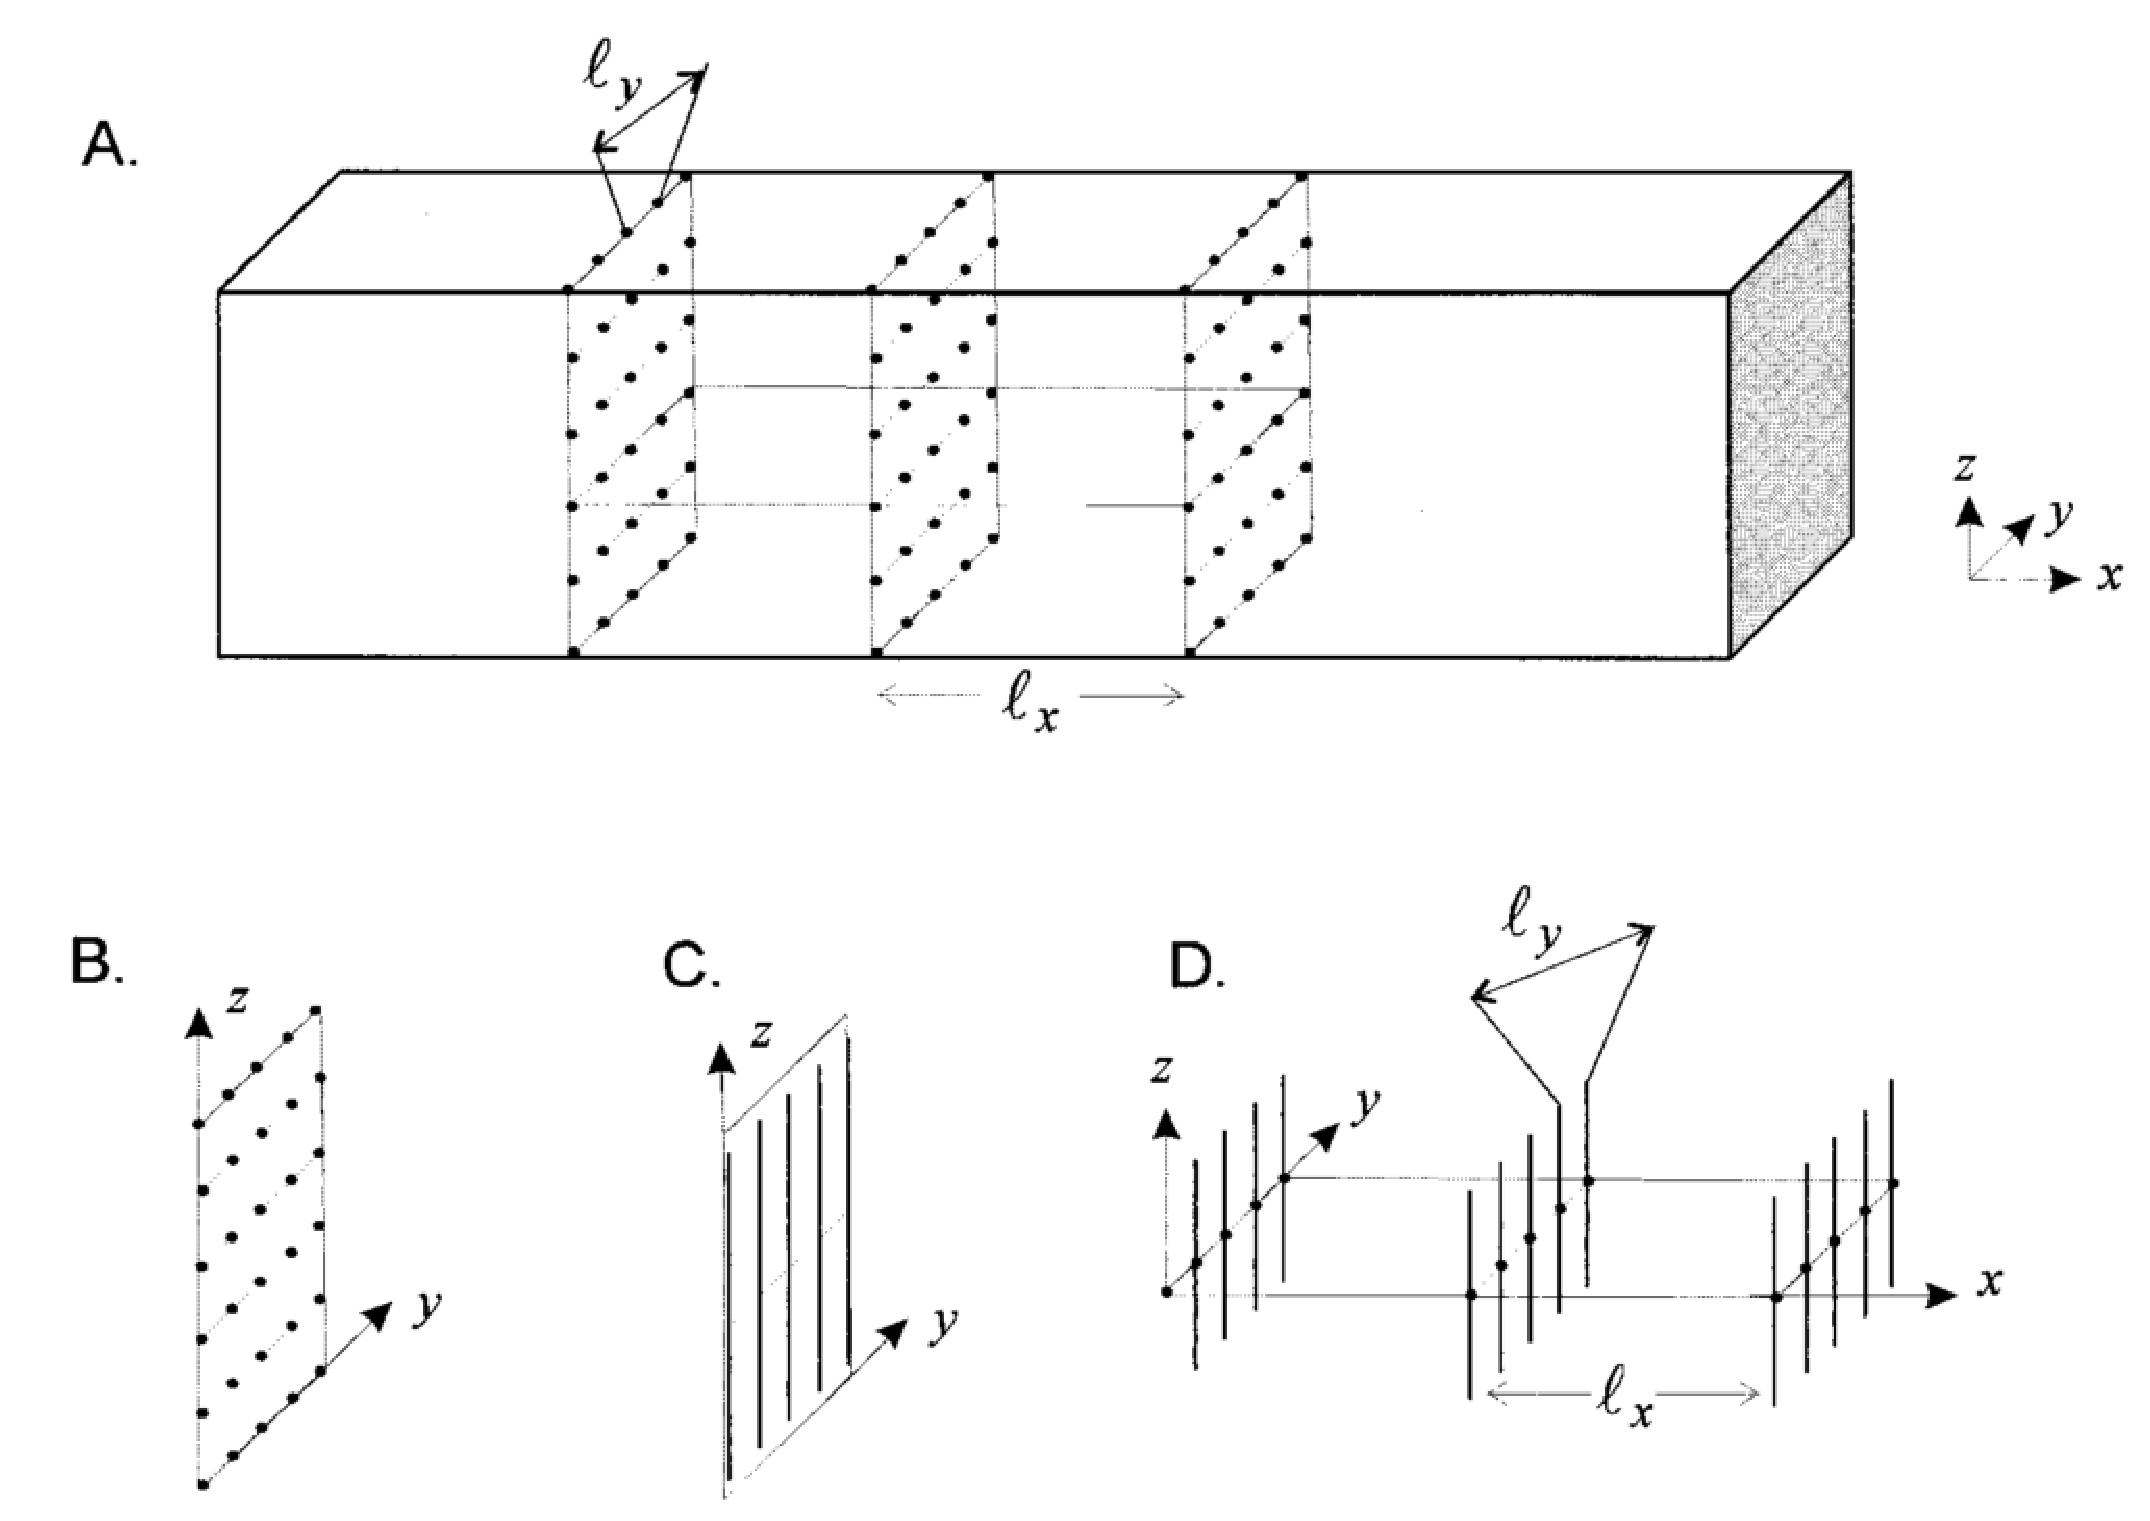
\includegraphics[height=5cm,
    angle=0]{./images/Izu_2001_cell.eps}}
\caption{A 3D schematic diagram of cardiac ventricular cell. Z-lines
  are spaced at a distance 2$\mu$m apart in x-direction. They yz-plane
  at each z-line contains the CRU (the dots).}
\label{fig:Izu_cell}
\end{figure}

$\Ca$ release from the CRU will generate concentration gradient in
all directions. However, for simplicity, they eliminate the
z-direction and thus model the calcium release on a single z-line
only. In other words, the CRU release in the z-direction is assumed
to extend infinitely, making planes at any z-line equivalent. 


The inter-CRU distance on y-axis are simulated with 0.4$\mu$m and
0.8$\mu$m. 
\section{Okada-...-Hisada (2005)}
\label{sec:okada-...-hisada}

~\citep{okada2005}


\section{Shiferaw-Karma (2006)}
\label{sec:shiferaw-karma-2006}

(An introduction to cardiac alternans is described in
Sect.~\ref{sec:card-cell-altern}).  

~\citep{Shiferaw2006} proposed an amplitude equation, describing the
coupled dynamics of intracellular calcium and membrane voltage. The
prediction for the formation of SDA is {\it Turing instability}.
Turing, in 1952, discovered that
\textcolor{red}{the interaction of two substances with different
  diffusion rates can generate spatial concentration patterns starting
  from near-uniform spatial distribution}.
Turing used Fourier-type stability analysis of linear equations based
on the amplification of waves with certain spatial wave-lengths after
small perturbation.

The simplest system has two variables: an activator and an inhibitor.
So, what about pattern formation with systems having more than 2
variables~\citep{Meinhardt2000} which is the most common.

\subsection{Hypothesis analysis}
\label{sec:hypothesis-analysis-13}

A spatial model is built by dividing the cell into sections.
A typical ventricular myocyte has length 150$\mu$m, with diameter
20$\mu$m, containing 75-100 sarcomere,
Fig.~\ref{fig:Shiferaw_Karma}. So, they divided the cell into
subunits, each one corresponds to a single sarcomere. Eventually, the
cell is modeled as a 1D chain of these identical subunits. Another
assumption is that the $\Ca$ diffusion is fast enough on the scale of
a single sarcomere that $[\Ca]$ in a subunit is uniform. 

\begin{figure}[hbt]
  \centerline{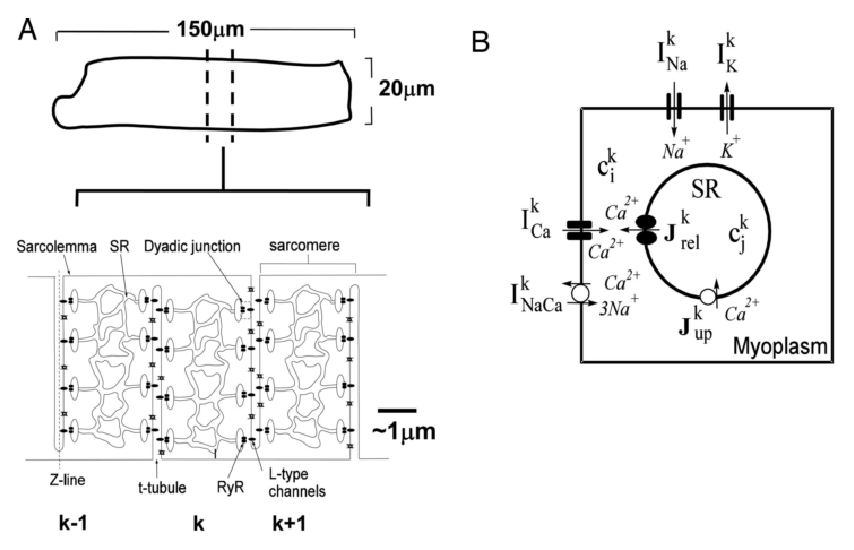
\includegraphics[height=6cm,
    angle=0]{./images/Shiferaw_Karma.eps}}
 \caption{(A) Schematic representation of a cardiac cell; (B) Ca
   cycling machinery that regulate $V_m$ within a sarcomere}
\label{fig:Shiferaw_Karma}
\end{figure}

\subsubsection{$V_m$ dynamics}
\label{sec:v_m-dynamics}

The effective diffusion of voltage is $D_V=2.5\times10^{-4}$cm$^2$/ms
or 25000$\mu$m$^2$/ms.  So, $V_m$ equilibrates rapidly over the length
scale of the cell on the time scale of about 0.5ms, which is
comparable with the rise time of AP (i.e. 1ms), but much smaller than
AP duration (APD). So, they assume all sarcomeres sense the same $V_m$
(\textcolor{red}{This is no longer accurate if we use exact method
  that requires very small time step}).

The ionic currents for each subunit are shown in
Fig.~\ref{fig:Shiferaw_Karma}. 
\begin{enumerate}
\item $I^k_\Na$: fast inward Na current

\item $I^k_\K$: total outward K current

\item $I^k_\Ca$:

\item $I^k_\NaCa$:  
\end{enumerate}
The formula for all ionic currents are based on~\citep{fox2002}
(Sect.~\ref{sec:fox-mcharg-gilmour}). 

\subsection{Mathematical model}
\label{sec:mathematical-model-19}

\begin{equation}
  \label{eq:1047}
  C_m\frac{dV_m}{dt} = -\sum_{k=1}^N (I^k_\na+I^k_\ca+I^k_\K+I^k_\NaCa)+I_{app}
\end{equation}
with $N$ is the number of sarcomere units in this case.




\section{Li-Lancaster-Holden (2007) ventricular E-cell}
\label{sec:li-lancaster-holden}

E-cell is a project launched in 1996 to recreate cellular phenomena in
silico~\citep{tomita1999}.

\subsection{Hypothesis analysis}
\label{sec:hypothesis-analysis-19}


~\citep{li2007} created a realistic geometrical model of ventricular
myocyte (3Dv E-cell) as a cylinder with diameter 16$\mu$m, and length
of 100$\mu$m with the space step is 0.2$\mu$m, i.e. the cell volume is
about 20.1pL. It means the image in voxels is 80x80x500 matrix with
3.2 million grid points, Fig.~\ref{fig:Li_3Dcell}(c).

\begin{figure}[hbt]
  \centerline{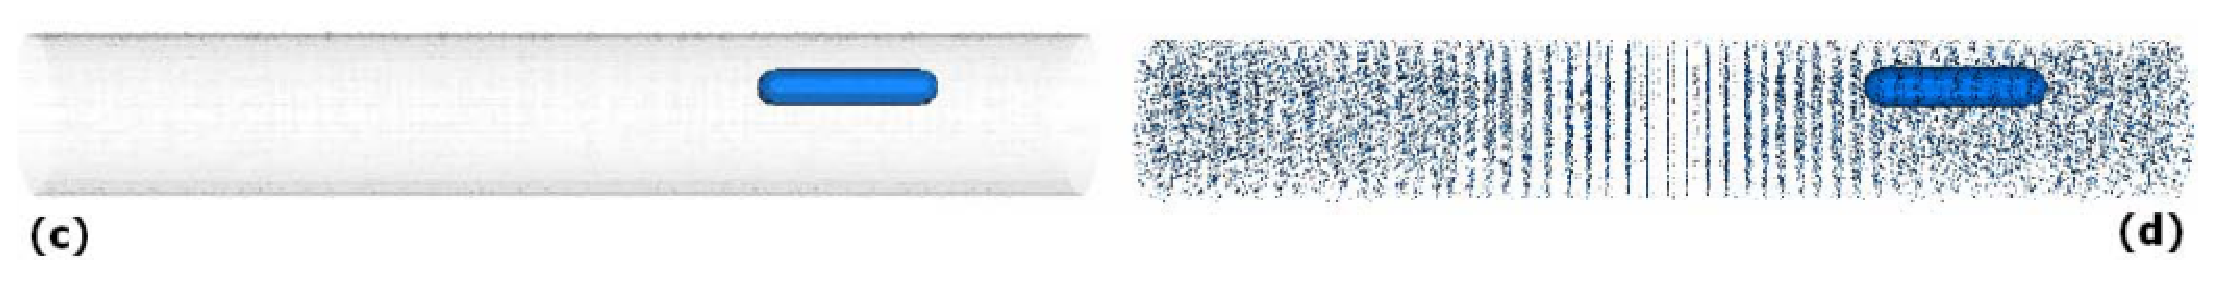
\includegraphics[height=1.5cm,
    angle=0]{./images/Li_3Dcell.eps}}
  \caption{ (c) A cylinder diagram of the 3Dv E-cell, with nucleus
    (blue), (d) RyRs clusters are randomly distributed}
\label{fig:Li_3Dcell}
\end{figure}

Based on~\citep{chen-izu2006tdd}, resting state spacing between
neighboring Z-disks is $1.87\pm0.18\mu$m. RyR clusters are
``randomly'' distributed, Fig.~\ref{fig:Li_3Dcell}(d), with transverse
spacing of $1.05\pm0.44\mu$m, and longitudinal spacing of
$0.83\pm0.31\mu$m. For peripheral RyR clusters, their spacing is
$1.97\pm0.42\mu$m.

The density is 0.4/$\mu$m$^2$ is used for cell surface.~\citep{li2007}
also incorporated a nucleus with diameter of 5.0$\mu$m and length of
10$\mu$m, with its center is located 20$\mu$m from the end, and
5$\mu$m from the surface of the cell. 

Assumptions:
\begin{enumerate}
\item $\Ca$ release from CRU is considered as a point source
  $i_\ca=2$pA. The release time $\tau=10$ ms pulse. So, the total
  amount of calcium release is $(\sigma_\ryr\times\tau)$. To model the
  wave, they keep the $[\Ca]_i$ low and use a much larger point source
  $i_\ca=8$pA. 
  \begin{equation}
    \label{eq:1359}
    \sigma_\ryr = \frac{i_\ca}{z_\ca F} \;\;\; \text{[mol/s]}
  \end{equation}

\item Calcium buffers, and SR are considered to be uniformly
  distributed over the geometry.

\item Diffusion coefficients of free calcium are anisotropic:
  $D_{c,x}$=300$\mu$m$^2$/s along the cell, and $D_{c,y/z}=$150$\mu$m$^2$/s in
  transversal direction.

\item There is no mobile buffer. The 2 immobile buffers are:
  calmodulin (CaM) and Troponin C (TrpnC).

\item mathematical description is based on~\citep{izu2001}


\item SERCA pump is based on the classical Hill equation,
  eq.~\eqref{eq:1357}
\end{enumerate}
\begin{equation}
  \label{eq:1361}
  J_i = -\frac{\partial [\CaBi]}{\partial t}
\end{equation}
with $i$ can be CaM and trpnc. 
\begin{equation}
  \label{eq:1363}
  J_i = k^-_i[\CaBi] - k^+_i[\Ca]_\myo([\Bi]_T - [\CaB_i])
\end{equation}

\subsection{Mathematical analysis}
\label{sec:math-analys-3}

\begin{enumerate}
\item Calcium dynamics
  \begin{equation}
    \label{eq:1355}
    \frac{\partial [\Ca]_\myo}{\partial t} = \nabla \cdot (D_c
    \nabla[\Ca]_\myo) + J_{sum}
  \end{equation}
with 
\begin{equation}
  \label{eq:1356}
  J_{sum} = J_\ryr + J_\leak - J_\serca + J_\buf
\end{equation}
with $J_\buf$ is in the direction of releasing $\Ca$.
\begin{equation}
  \label{eq:1357}
  J_\serca=v_\serca \frac{([\Ca]_\myo)^\eta}{K_{m,\serca}^\eta+([\Ca]_\myo)^\eta}
\end{equation}
with $v_\serca=200\mu$M/s, $K_{m,\serca}=0.184\mu$M.

The leak is set to balance the uptake at resting
\begin{equation}
  \label{eq:1358}
  J_\leak = J_\serca(c_o)
\end{equation}
with $c_o=0.1\mu$M is the resting concentration of $[\Ca]_\myo.$
\begin{equation}
  \label{eq:1360}
  J_\ryr = \sigma_\ryr \delta(\mathbf{r})
\end{equation}
with $\delta(\mathbf{r})$ is the magnitude of the current at a
distance $\mathbf{r}$ from the point source. 
\begin{equation}
  \label{eq:1362}
  J_\buf = \sum J_i
\end{equation}

\item Calcium release from a single CRU: as a point source, it has 2
  states S = 0 (resting) or 1 (firing). To determine the state, a
  uniformly distribution pseudo-random number $u_\rand$ is withdrawn
  for each CRU. This value will be used to compare with the
  probability $P_o$ which is calculated from $[\Ca]_\myo$ and
  $\Ca$-sensitivity $K_{poss}$.
  \begin{equation}
    \label{eq:1364}
    P_o = \frac{([\Ca])^n}{(K_{poss})^n + ([\Ca]_\myo)^n}
  \end{equation}
with $n=1.6$; and
\begin{itemize}
\item S=1 if $P_o>u_\rand$
\item The starting time for the N-th spark at site M: $T^M_N$ should
  satisfy $T^M_N > T^{M-1}_N + \tau_R$ (with $\tau_R$ is the
  refractory period)
\end{itemize}


\item Data for buffers
\begin{table}[hbt]
\begin{center}
\caption{$\Ca$ buffers}
\begin{tabular}{ccccc} 
  \hline
  & $k^+_i$ (1/($\mu$M.s))& $k^-_i$ (1/s) $[\Bi]_T$ & $K_i$ \\ 
  \hline\hline
  CaM & 100 & 38 & 24 & 0.38 \\
  TrpnC & 39 & 20 & 70 & 0.51
\end{tabular}
\end{center}
\label{tab:Li2007_buffers}
\end{table}

\end{enumerate}

\subsection{Numerical analysis}
\label{sec:numerical-analysis-3}

They use finite difference method with space step 0.2$\mu$m, and time
step 10$\mu$s. Zero-flux boundary conditions are implemented, by
setting the value of $[\Ca]_\myo$ at the boundary points to be the
same as their immediate internal neighbors.

Simulation is conducted on SunBlade 2000 workstations, with initial
conditions setting at rest and $c_o=0.1\mu$M

\subsection{Data analysis}
\label{sec:data-analysis-5}

They perform simulation in 2D with width 28$\mu$m and height 100$\mu$,
which gives a lattice of $140\times500=70000$ grid points. They don't
have any 3D simulation at all. So the question whether this is
reliable????

The wave can only be triggered with a large current $i_\ca=8$pA and
$K_{poss}=1000\mu$M. NOTE: Using $i_\ca=5$pA, $K_{poss}=800\mu$M, wave
failed to propagate. 


 Reentrant $\Ca$ spiral waves can be initiated using
 \begin{itemize}
 \item S1-S2 protocol
 \item wave cutting
 \item propagation through heterogeneity (or around obstacles)
 \end{itemize}
In the model, the nucleus serves as the obstacles that lowering the
diffusion. If the wave is initiated closed to the nucleus, with
$i_\ca=5$pA, $K_{poss}=800\mu$M, $\tau=10$ms, $\tau_R=350$ms.

\subsection{Related papers}
\label{sec:related-papers}

~\citep{li2009} use a smaller size of the cell: 24$\mu$m$\times
24\mu$m$\times 7.2\mu$m which was discretized into 120$\times
120\times 36$ voxels. It means each voxel is of size $0.2\mu$m$\times
0.2\mu$m$\times 0.2\mu$m.

Experimental data show that Z-disks do not flat on the transversal
surface, but forming an angle with the transversal axis,
e.g. 7.6$^\circ$. 
\begin{figure}[hbt]
  \centerline{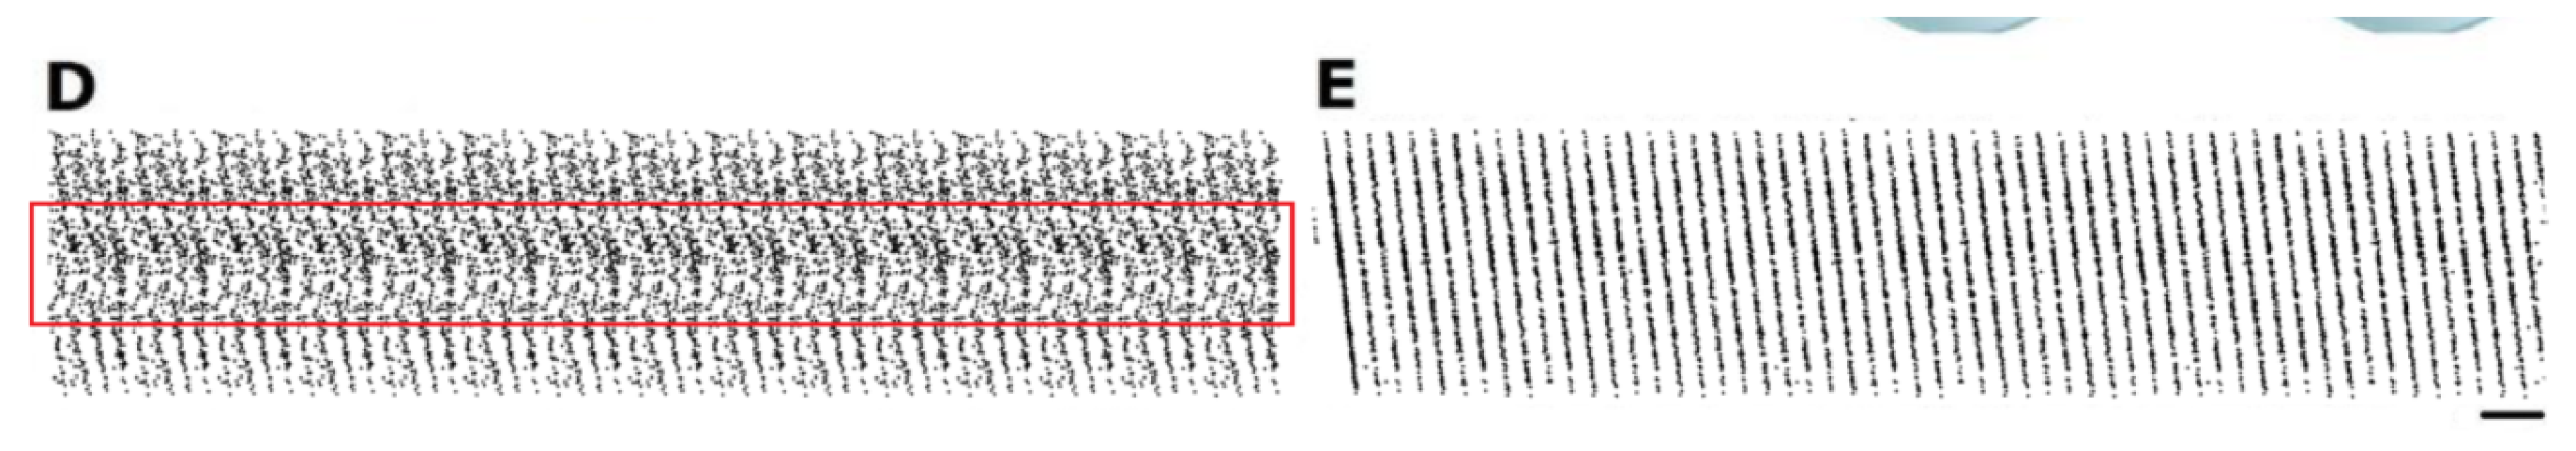
\includegraphics[height=2cm,
    angle=0]{./images/Li_Zdisk.eps}}
  \caption{3.5 Z-disks repetitively in the longitudinal direction, (E)
    RyR clusters in 2D planes forming an angle of 7.6$^\circ$ to the
    transversal axis. Scale bar is 5$\mu$m. Redbox indicates the
    bifurcation region}
\label{fig:Li_Zdisk}
\end{figure}



\section{Soeller-...-Cannell (2009) rat ventricular myocyte}
\label{sec:soeller-...-cannell}

This model is based on the previous work of ~\citep{li2007}
(Sect.~\ref{sec:li-lancaster-holden}). 

\subsection{Testing methods}
\label{sec:testing-methods}

\begin{enumerate}
\item Initially set the $[\Ca]_\myo$ to 50$\mu$M in a small region,
  which can robustly initiate calcium waves~\citep{soeller2008}. Lower
  values may failure to initiate the waves.
\end{enumerate}

\subsection{Numerical solving}
\label{sec:numerical-solving-3}

A numerical solver was written in C, and simulation was performed on
Lenovo T61P laptop with 2.5GHz Intel Core2 Duo and 4GB. It took 3h to
simulate 500ms. 

%%% Local Variables: 
%%% mode: latex
%%% TeX-master: "mainfile"
%%% End: 
